% search all chinese words with regex:  [一-龥]+

% \usepackage{nextpage} % for starting on odd number pages (\clearpage, \newpage)
% \usepackage{sectsty} %styling of section headers
% \usepackage{array} % for tables

% \hyphenation{
%   Afri-can Afri-cans afri-ca-nus
%   Ara-fura
%   Ata-huallpa
%   Caja-marca
%   Chal-cu-chima
%   Chat-ham Chat-hams
%   Colum-bia Colum-bian
%   Cui-tla-huac
%   Dingi-swayo
%   Gui-nea Gui-neans
%   Kame-ha-meha
%   Lin-e-ar-band-ke-ramik
%   Meadow-croft
%   Medi-ter-ra-nean
%   Men-in-dee
%   Mes-o-po-ta-mia Mes-o-po-ta-mian
%   Molo-kai
%   Mon-te-zuma
%   Mori-ori
%   Reichs-kom-mis-sar
%   Sas-katch-e-wan
%   Span-iard Span-iards
%   Tenoch-ti-tlan
%   Tut-ankh-a-men
%   Vil-ca-shu-a-man Vil-ca-conga
%   Vira-co-cha
%   Wind-hoek
%   archi-pel-ago archi-pel-a-goes
%   blue-print blue-prints
%   clam-shell clam-shells
%   cor-vee cor-vees
%   dipro-to-dont dipro-to-donts
%   entre-pre-neur-ial
%   for-mi-da-ble
%   her-maph-ro-dite her-maph-ro-dites
%   life-style life-styles
%   mega-fauna
%   pome-gran-ate pome-gran-ates
%   pro-gress
%   scru-tiny
%   spe-cies
%   teo-sinte
%   wide-spread
% }

% custom:
% article{texblog2012,
%   keywords = {own}, % keyword for subdivided bibliography
%   title={My fancy publication},
%   author={Texblog, T},
%   journal={TUGboat},
%   volume={33},
%   number={3},
%   pages={1001--1002},
%   year={2012},
% }
% \printbibliography[keyword=own,...]
% \printbibliography[notkeyword=own,...]



% \begin{tcolorbox}[breakable, enhanced]



% ch: 	chapter
% sec: 	section
% subsec: 	subsection
% fig: 	figure
% tab: 	table
% eq: 	equation
% lst: 	code listing
% itm: 	enumerated list item
% alg: 	algorithm
% app: 	appendix subsection 

% Lorem ipsum \tikz\draw [thick,dash dot] (0,0) -- (3,0); dolor sit amet

% Lorem ipsum \tikz[baseline=-0.5ex]\draw [thick,dash dot] (0,0) -- (3,0); dolor sit amet



% \cleardoublepage
% \printbibheading
% \printbibliography[heading=subbibliography, title={Book references},type=book]
% \printbibliography[heading=subbibliography, title={Article references},type=article]
% \printbibliography[heading=subbibliography, title={Dictionary entries}, nottype=article, nottype=book]



% \begin{figure}[!hbt]
%     \centering
%     \subfloat[\centering \textit{aaa}]{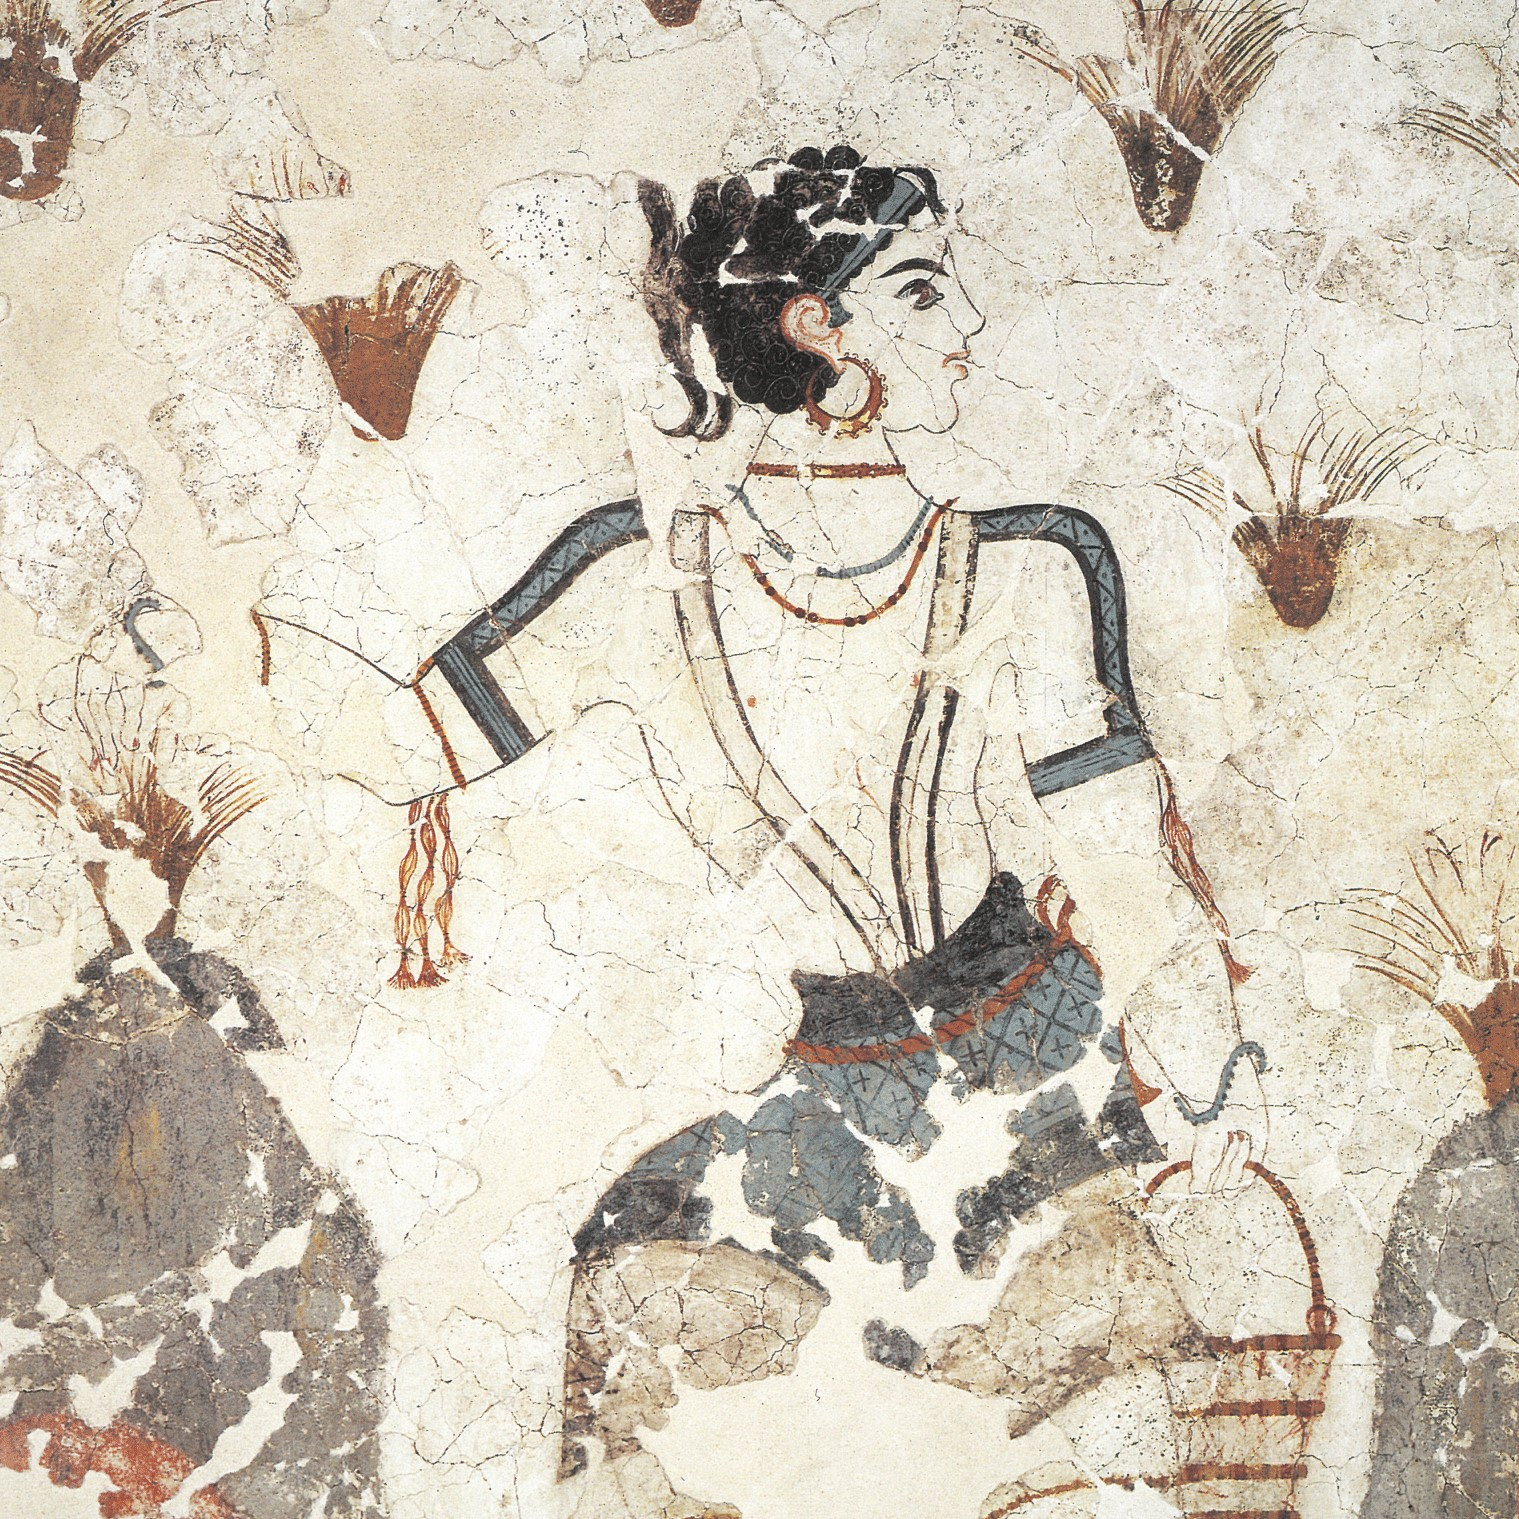
\includegraphics[width=0.475\linewidth]{imgs/saffron_gatherers_l.jpg}}
%     \hfill
%     \subfloat[\centering \textit{bbb}]{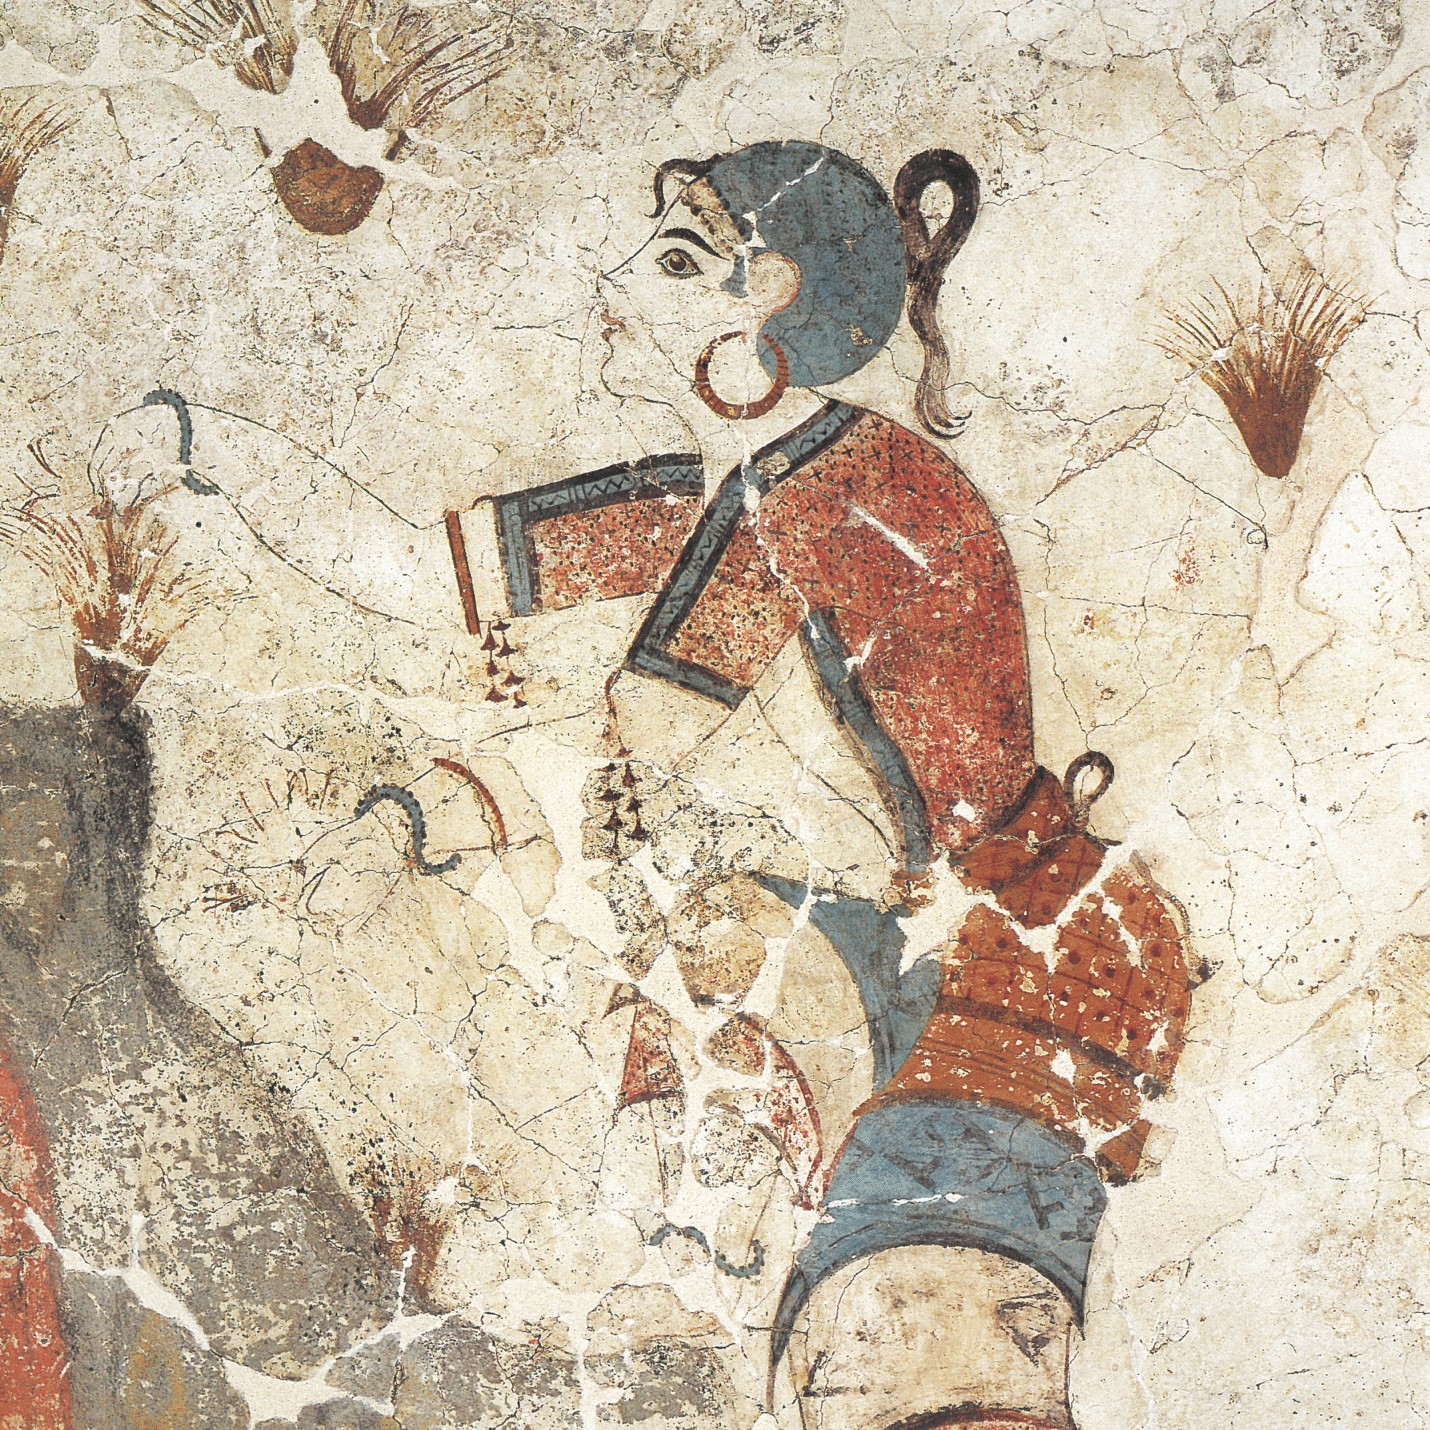
\includegraphics[width=0.475\linewidth]{imgs/saffron_gatherers_r.jpg}}
%     \caption{Saffron-gatherers. Details from the mural on the east wall in room 3a, first floor at Xeste 3 site \autocite[152]{doumas_wall-paintings_1992}}
%     \label{fig:saffron_gathererss}
% \end{figure}


% \begin{appendices}
% \chapter{Appendix Alpha}
% \section{Section Alpha}
% The contents...
% \end{appendices}


% \usepackage[a4paper]{geometry}
% \usepackage[
%     a4paper,
%     nohead,
%     includefoot,
%     includemp,
%     bindingoffset=0.5cm,
%     top=2.25cm,
%     left=3.75cm,
%     right=0.75cm,
%     bottom=1.5cm,
%     marginparwidth=1.75cm,
%     marginparsep=10pt,
%     footskip=2cm,
% ]{geometry}


% % Extend the list of base directories
% \makeatletter
% \def\input@path{{imgs/}{imgs/logos/}{utils/}{contents/}{fonts/}}
% \makeatother



% indexing
% \subsubsection{The back of your bra rides up towards your shoulder}
% If the back of the bra rides up towards your shoulder blades it usually
% indicates the back of the bra is too big. For example – if you are wearing
% a 36C, it may be worth trying a 34D or even a 32DD. (Take a look at our
% bra sizing guide to help you with this.) 
% \index{Bra|textbf} 
% % \index{\textbf{Bra}|textbf} 

% \subsubsection{The bra cup digs into your bust at the top creating a ‘double-bust’ effect}
% If the bra cups digs into your bust at the top, it is a sure sign that
% the bra cup is too small. Try the next cup size up! 
% \index{Bra!classic}
% \index{Bra!standard}

% \begin{wrapfigure}{O}{0.5\textwidth}
%   \includegraphics[width=0.5\textwidth,trim=0cm 0cm 0cm 0cm,clip]{thesis/imgs/toppng.com-green-chili-peppers-1470x1095.png}
%   \caption{Allspice}
% \end{wrapfigure}

% \DeclareTextFontCommand{\newcommand}{\cuneiform}



%%% Simple multi-line cells
% \newcommand{\cell}[1]{\begin{tabular}{@{}l@{}}#1\end{tabular}}
% \newcommand{\ccell}[1]{\multicolumn1c{\begin{tabular}{@{}c@{}}#1\end{tabular}}}

%%% Empty cells in tables
% \newcommand{\na}{\hspace{1em}---}


% ...⟪ ⟫...《…》... second one is chinese title mark 《Bencao Gangmu》
